\chapter{\dspot: A Test Amplification Tool}
\label{chapter:dspot}

\begin{chaptersummary}
		In this chapter, I expose the major output of this thesis. \dspot is a test amplification tool that have the ambition to improve the test suite of real projects, and the global quality of continuous integration process.
		\dspot achieves this by providing a set of automated procedures, and work at two majors levels:\\
		1) it amplifies the test suite offline, and the outputted amplified test methods can be used to growth and improve in the project's test suite;\\
		2) it amplified the test suite inside the Continuous Integration to enhance the developers' confidence in their changes, or increase the ability of the test suite to detect potential regression.
\end{chaptersummary}

\minitoc

\graphicspath{{.}{chapitres/dspot/}}

% ---------------------------------------------------------------------------------------
% definitions
% ---------------------------------------------------------------------------------------
\section{Definitions}

We first define the core terminology of \dspot in the context of object-oriented Java programs.

\textbf{Test suite} is a set of test classes.

\textbf{Test class} is a class that contains test methods. A test class is neither deployed nor executed in production.

\textbf{Test method} or \textbf{test case} is a method that sets up the system under test into a specific state and checks that the actual state at the end of the method execution is the expected state.

\textbf{Unit test} is a test method that specifies a targeted behavior of a program. 
Unit tests are usually independent from each other and execute a small portion of the code, \ie a single unit or a single component of the whole system.

\textbf{System test} or \textbf{Integration test} is a test method that specifies a large and complex behavior of a program.
System tests are usually large, long to be executed and use a lot of different component of the program.

\textbf{Test-criterion} is a measure of the quality of the test suite according to an engineering goal.
For instance, one can measure the execution speed of its test suite, and consider that the faster it is executed the better it is.
The most popular would be probably the execution coverage, which can be measured a different level: branches, statements, instructions.
It measures the proportion of the program that the test suite executes.
The more it executes, the better is considered the test suite since it is likely to verify more behavior.

\textbf{Amplified test suite} is an existing test suite to which we add amplified test methods.

\textbf{Amplified test method} is a test method that has been amplified, \ie it has been obtained using an test amplification process and an existing test method.

\textbf{Test input} is the first key component of test methods. 
It is responsible to set the program into a specific state using objects, method calls and literals.

\textbf{Assertion} or \textbf{oracle} is the second key component of test methods. 
It is responsible to verify that the state of the program, when the test input (the first component) is executed, is the expected one. 
It takes the form of comparison between hard-coded values and program's values, or the presence / absence of errors.

\section{Principle}
\label{sec:dspot:principle}

\begin{figure}[h]
	\centering
	\fbox{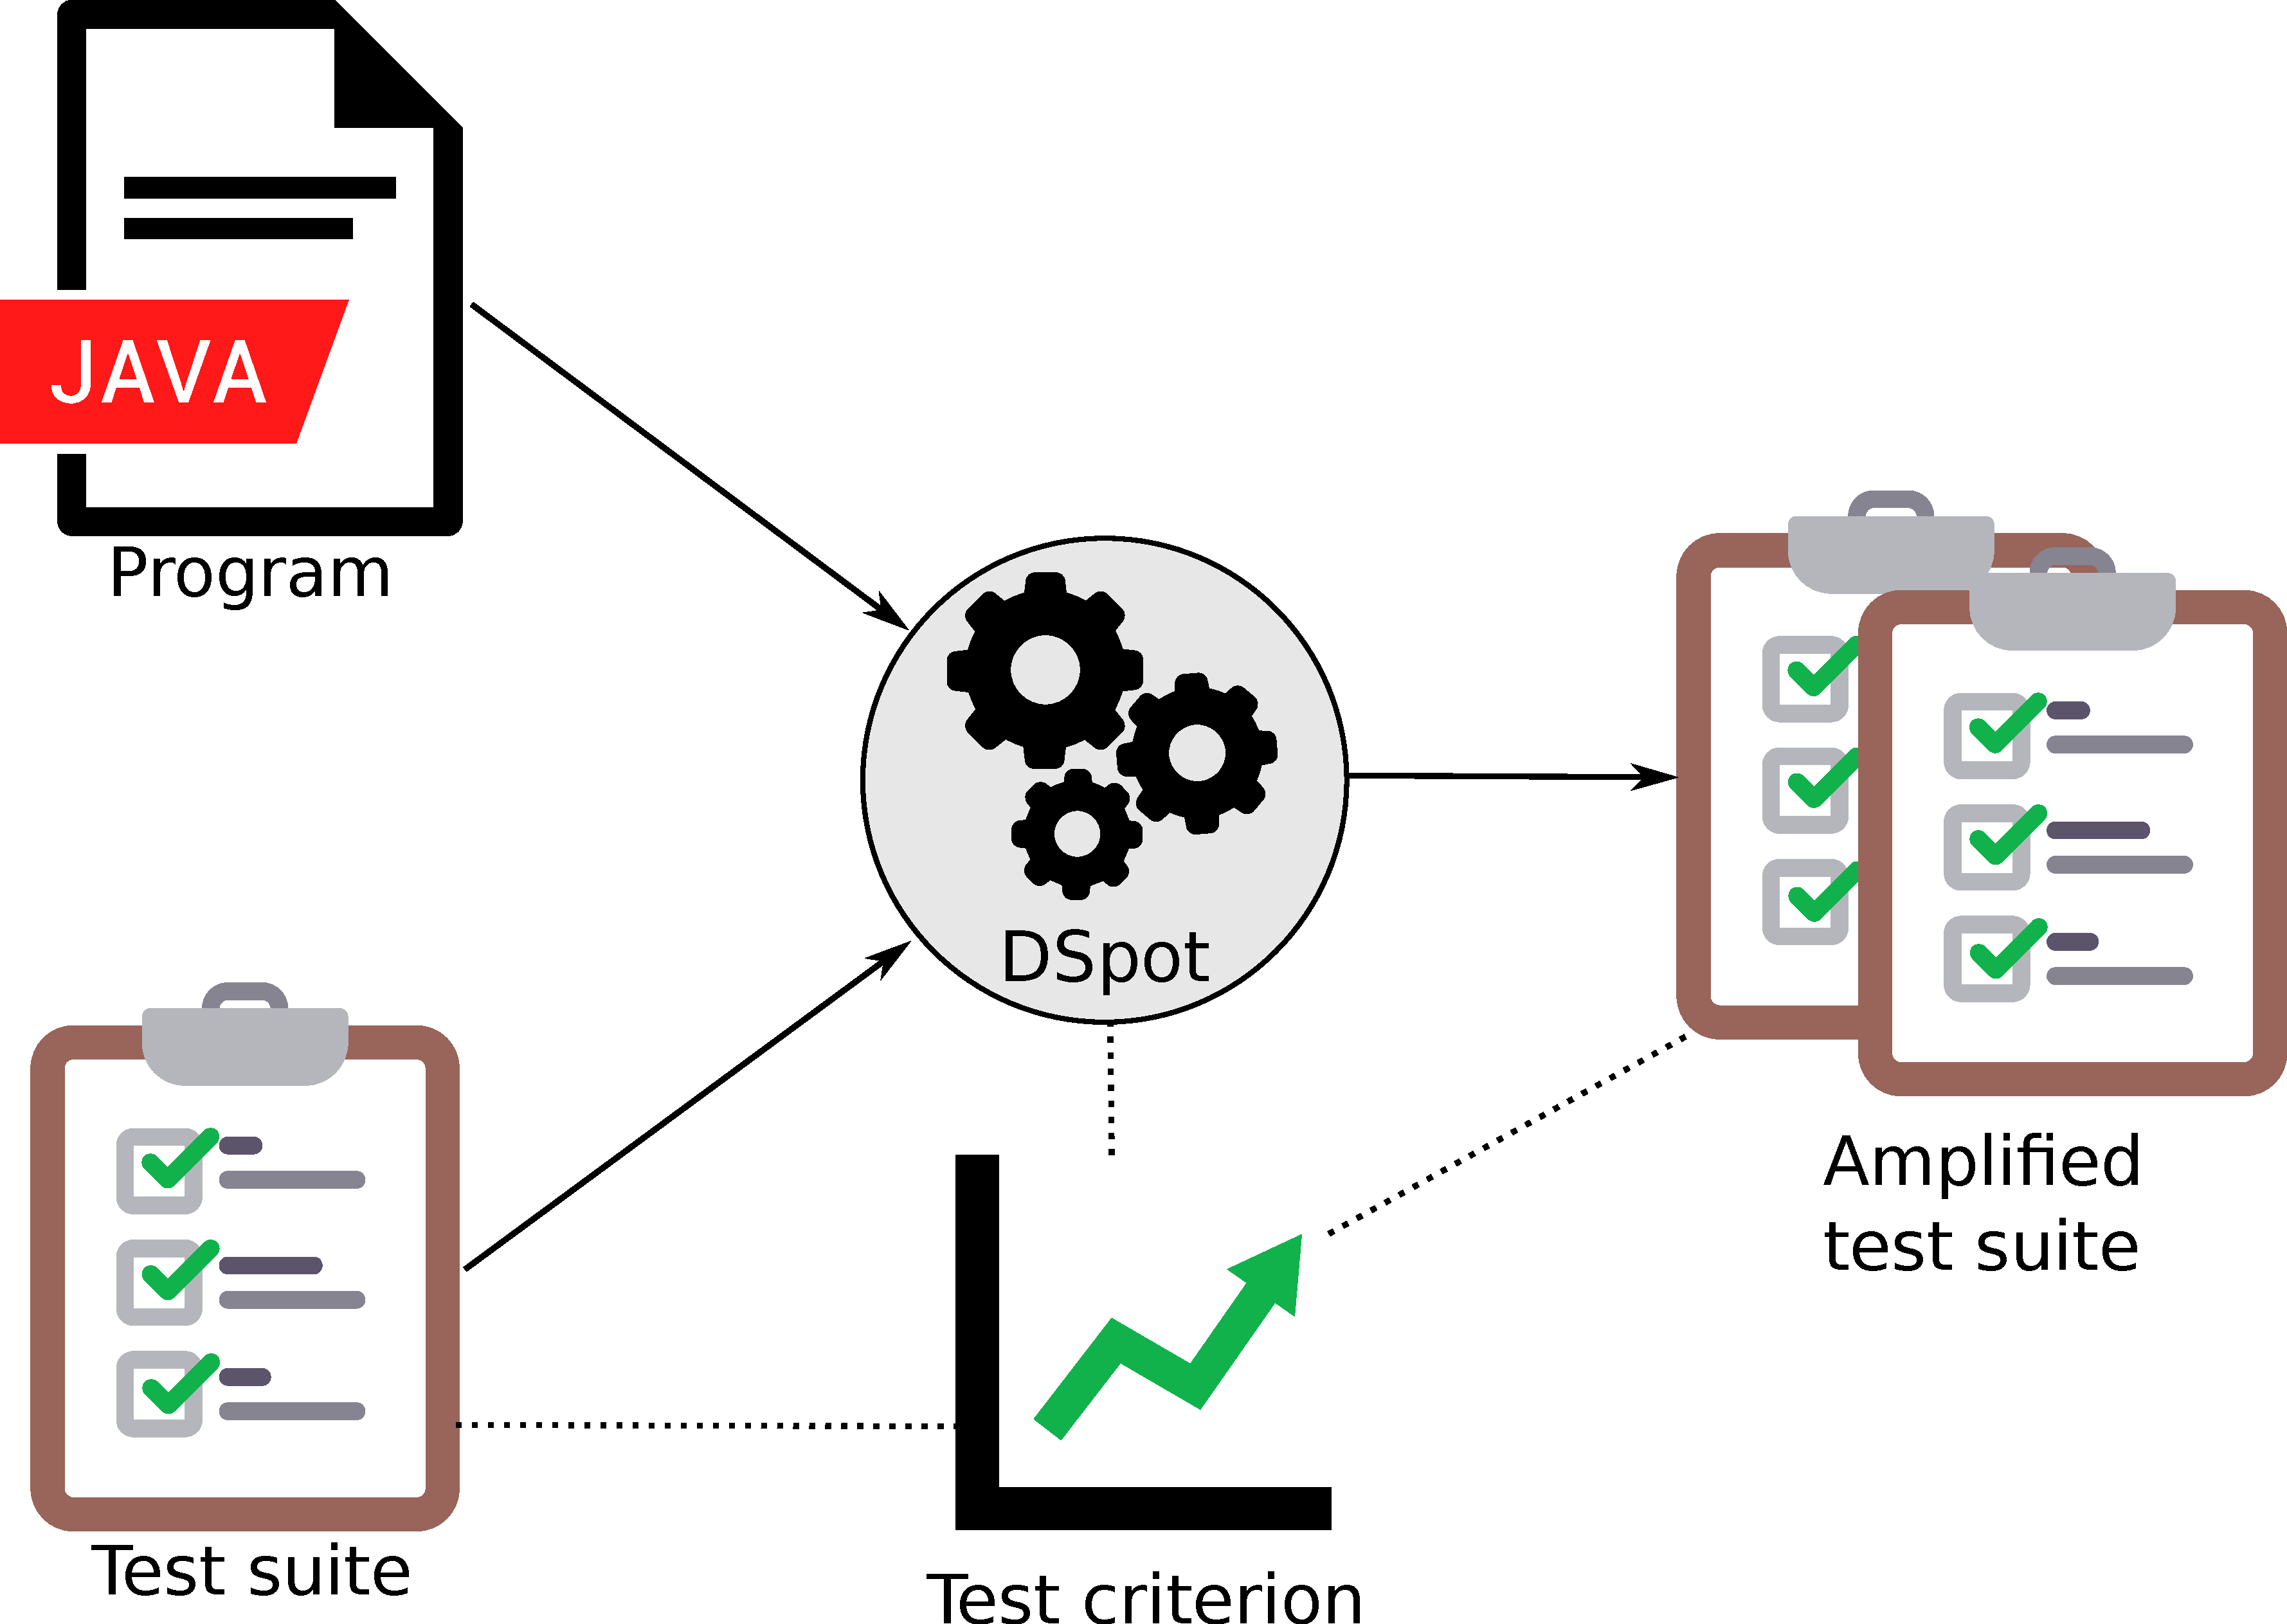
\includegraphics[width=.6\linewidth]{dspot_principle.pdf}}
	\caption{
		\dspot's principle: \dspot takes as input a program, an existing test suite, and a test-criterion. 
		\dspot outputs a set of amplified test methods.
		When added to the existing test suite, these amplified test methods increase the test-criterion, \ie the amplified test suite is better than the original one.
	}
	\label{fig:dspot:principle}
\end{figure}

DSpot is a test amplification tool.
Its goal is to improve an existing test suite according to a specific test-criterion.
DSpot takes as input the program, an existing test suite, and a test-criterion. 
The output of DSpot is a set of amplified test methods that are variants of existing test methods.
When added to the existing test suite, it create an \emph{amplified test suite}.
This amplified test suite is better than the original test suite according to the test-criterion used during the amplification.
For instance, one amplifies its test suite using branch coverage as test-criterion.
This amplified test suite will execute more branches than the exiting test suite, \ie the one without amplified test methods.

\dspot's principle is summarize in \autoref{fig:dspot:principle}.

\section{Algorithm}
\label{sec:dspot:algorithm}

\subsection{Input}
\label{subsec:dspot:algorithm:input}

\dspot's inputs are a program, a set of existing test methods and a test-criterion.
The program is used as ground truth: in \dspot we consider the program used during the amplification correct.
The existing test methods are used as a seed for the amplification.
\dspot applies transformation individually to these test methods in order to improve the overall quality of the test suite with respect to the specified test-criterion.

\subsection{Output}
\label{subsec:dspot:algorithm:output}

\dspot produces variants of the test methods provided as input.
We call these variants \emph{amplified test methods}, since there are test methods that has been obtained using an amplification process.
These amplified test methods are meant to be added to the test suite.
By adding amplified test methods to the existing test suite, it creates an amplified test methods that improve the overall test suite quality.
By construction, the amplified test suite is at least as good, or better than the original one with respect to the specified criterion.

An amplified test method's integration can be done in two way:
1) the developer integrates as it is the amplified test method into the test suite;
2) the developer integrate only the changes between the original test method and the amplified test method.
This enrich directly an existing test method.

\begin{figure}[h]
	\centering\fbox{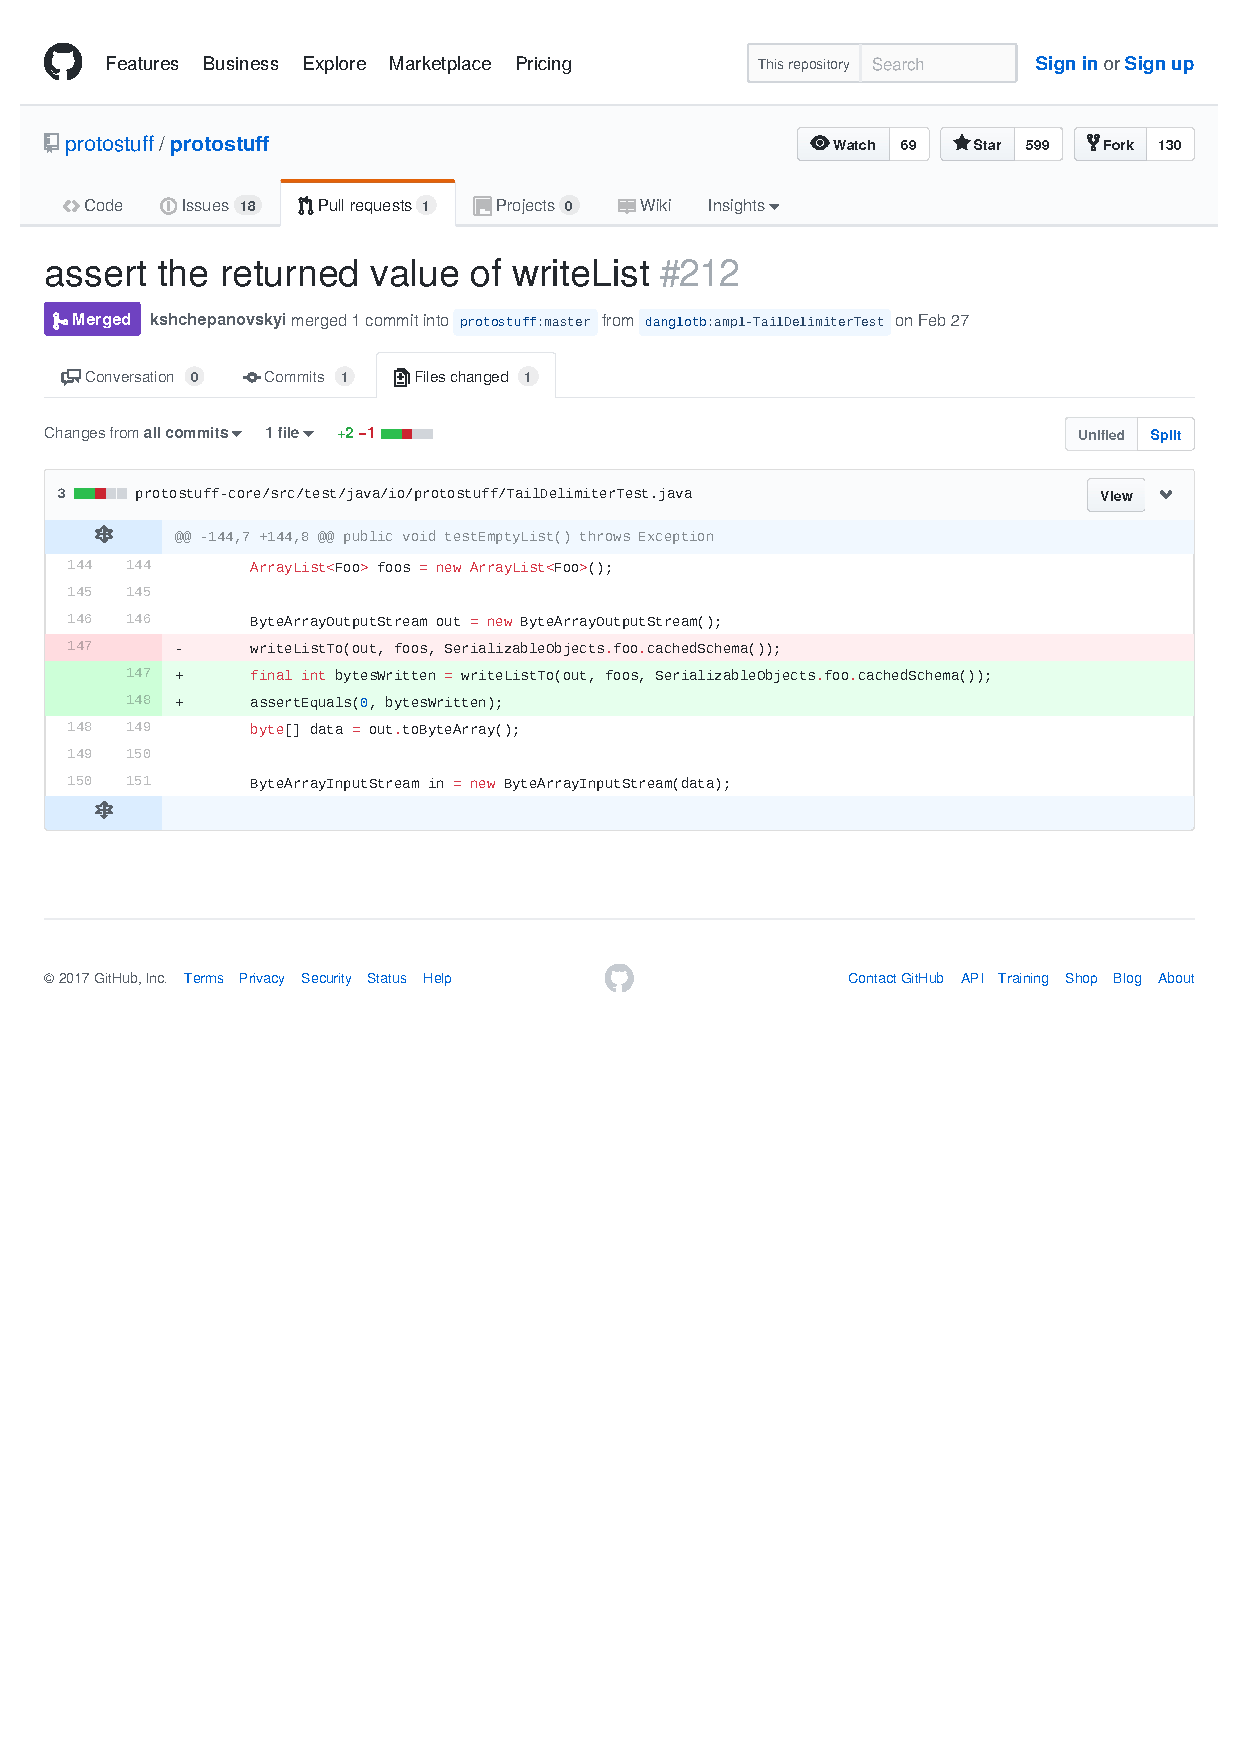
\includegraphics[width=0.98\textwidth, trim=4.15cm 17.52cm 4.05cm 10.76cm, clip]{protostuff.pdf}}
	\caption{Example of what \dspot produces: a diff to improve an existing test case.}
	\label{fig:diff-protostuff}
\end{figure}

\autoref{fig:diff-protostuff} shows an example of changes' set obtained using DSpot.

By construction, all \dspot's amplification can be represented as a diff on an existing test method since amplified test methods are variants of existing ones.

\subsection{Workflow}
\label{subsec:dspot:algorithm:workflow}

\begin{figure}[h]
	\centering\fbox{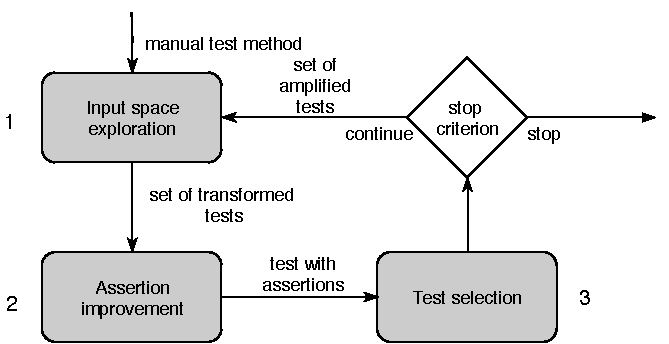
\includegraphics{dspot-workflow.pdf}}
	\caption{DSpot's workflow in three main steps: 1) the modification of test code's inputs, called ``input space exploration''; 2) the addition of new assertions called ``assertion improvement''; 3) the amplified test methods selection}
	\label{fig:dspot-workflow}
\end{figure}

The main workflow of \dspot is composed of 3 main phases:
1) the modification of test code's inputs inspired by Tonella's technique~\cite{tonella}, called ``input space exploration''; 
this phase consists in modifying test values (\eg literals), objects and methods calls, the underlying details will be explained in details in \autoref{subsec:dspot:algorithm:input-space-exploration}.
2) the addition of new assertions per Xie's technique~\cite{TaoXie2006}, this phase is called ``assertion improvement''.
The behavior of the system under test is considered as the oracle of the assertion, see \autoref{subsec:dspot:algorithm:new-assertions}.
In \dspot, the combination of both techniques, \ie the combination of input space exploration and assertion improvement is called ``test amplification''.
3) the amplified test methods selection according to a given test-criterion, \eg branch coverage.

\subsection{Modern Test Cases}
\label{subsec:dspot:algorithm:appliance-to-unit-test}

\begin{lstlisting}[caption={An example of an object-oriented test case  (inspired from Apache Commons Collections)},label=lst:archetype,float,language=java,numbers=left] 
testIterationOrder() {
// contract: the iteration order is the same as the insertion order

TreeList tl=new TreeList(); (*@\label{input-begin}@*)
tl.add(1);
tl.add(2); (*@\label{input-end}@*)

ListIterator it = tl.listIterator();(*@\label{test}@*)

// assertions
assertEquals(1, it.next().intValue());(*@\label{assertion-1}@*)
assertEquals(2, it.next().intValue());(*@\label{assertion-2}@*)
}
\end{lstlisting}

\dspot amplifies modern Java program's test methods, which are typically composed of two parts: test inputs and assertions. 
The input setup part is responsible for driving the program into a specific state.
For instance, one creates objects and invokes methods on them to produce a specific state.

The assertion part is responsible for assessing that the actual behavior of the program corresponds to the expected behavior, the latter being called the oracle.
To do so, the assertion uses the state of the program, \ie all the observable values of the program, and compare it to expected values written by developers.
If the actual observed values of the program state and the oracle are different (or if an exception is thrown), the test fails and the program is considered as incorrect.

\autoref{lst:archetype} illustrates an archetypal example of such a test case: 
first, from line \autoref{input-begin} to line \autoref{input-end}, the test input is created through a sequence of object creations and method calls; 
then, at line \autoref{test}, the tested behavior is actually triggered; 
the last part of the test case at \autoref{assertion-1} and \autoref{assertion-2}, the assertion, specifies and checks the conformance of the observed behavior with the expected one.
We note that this notion of call sequence and complex objects is different from test inputs consisting only of primitive values.

% ---------------------------------------------------------------------------------------
% input space exploration: INPUT GOAL
% ---------------------------------------------------------------------------------------
\section{Algorithms}

\subsection{Input Space Exploration Algorithm}
\label{subsec:input-space-exploration}

\dspot aims at exploring the input space so as to set the program in new, never explored states. To do so, \dspot applies code transformations to the original manually-written test methods. 

\textbf{I-Amplification:} \Iampl, for Input Amplification, is the process of automatically creating new test input points from existing test input points.

\dspot uses three kinds of \Iampl.

\emph{1) Amplification of literals}: the new input point is obtained by changing a literal used in the test (numeric, boolean, string).
For numeric values, there are five operators: $+1$, $-1$, $\times 2$, $ \div 2$, and replacement by an existing literal of the same type, if such literal exists.
For Strings, there are four operators: add a random char, remove a random char, replace a random char and replace the string by a fully random string of the same size.
For booleans, there is only one operator: negate the value;

\emph{2) Amplification of method calls}: \dspot manipulates method calls as follows:
\dspot duplicates an existing method call; removes a method call;
or adds a new invocation for an accessible method with an existing variable as target.

\emph{3) Test objects}:
if a new object is needed as a parameter while amplifying method calls, \dspot creates a new object of the required type using the default constructor if it exists.
In the same way, when a new method call needs primitive value parameters, \dspot generates a random value.

\dspot combines the different kinds of \Iampl iteratively: at each iteration all kinds of \Iampl are applied, resulting in new tests. 
From one iteration to another, \dspot reuses the previously amplified tests, and further applies \Iampl{}.

For example, if we apply an \Iampl on the example presented in \autoref{lst:archetype}, it may generate a new method call on \emph{tl}.
In \autoref{lst:iampl-example}, the added method call is ``removeAll''. Since \dspot changes the state of the program, existing assertions may fail. That is why it removes also all existing assertions.


\begin{lstlisting}[caption={An example of an \Iampl{}: the amplification added a method call to \emph{removeAll()} on \emph{tl}.},label=lst:iampl-example,float,language=java,numbers=left] 
testIterationOrder() {
TreeList tl=new TreeList(); (*@\label{input-begin-iampl}@*)
tl.add(1);
tl.add(2);
tl.removeAll();(*@\label{input-end-iampl}@*) // method call added

// removed assertions
}
\end{lstlisting}

% ---------------------------------------------------------------------------------------
% Assertion improvement
% ---------------------------------------------------------------------------------------
\subsection{Assertion Improvement Algorithm}
\label{subsec:new-assertions}

To improve existing tests, \dspot adds new assertions as follows.

\textbf{\Aampl:} \Aampl, for Assertion Amplification, is the process of automatically creating new assertions.

In \dspot, assertions are added on objects from the original test case, as follows: 
1) it instruments the  test cases to collect the state of a program after execution (but before the assertions), \ie it creates observation points. The state is defined by all values returned by getter methods.
2) it runs the instrumented test to collect the values,
the result of this execution is a map that gives, for each test case object, the values from all getters.
3) it generates new assertions in place of the observation points, using the collected values as oracle. The collected values are used as expected values in the new assertions.
In addition, when a new test input sets the program in a state that throws an exception,  \dspot produces a test asserting that the program throws a specific exception.

For example, let consider \Aampl{} on the test case of the example above. 

First, in \autoref{lst:aampl-example-1} \dspot instruments the test case to collect values, by addding method calls to the objects involved in the test case.

\begin{lstlisting}[caption={In \Aampl{}, the second step is to instrument and run the test to collect runtime values.},label=lst:aampl-example-1,float,language=java,numbers=left] 
testIterationOrder() {
TreeList tl=new TreeList(); (*@\label{input-begin-aampl}@*)
tl.add(1);
tl.add(2);
tl.removeAll();(*@\label{input-end-aampl}@*)

// logging current behavior
Observations.observe(tl.size()); 
Observations.observe(tl.isEmpty()); 
}
\end{lstlisting}

Second, the test with the added observation points is executed, and subsequently, \dspot{} generates new assertions based on the collected values. On \autoref{lst:aampl-example-2}, we can see that \dspot has generated two new assertions.

\begin{lstlisting}[caption={In \Aampl{}, the last step is to generate the assertions based on the collected values.},label=lst:aampl-example-2,float,language=java,numbers=left] 
testIterationOrder() {
TreeList tl=new TreeList(); (*@\label{input-begin-aampl2}@*)
tl.add(1);
tl.add(2);
tl.removeAll();(*@\label{input-end-aampl2}@*)

// generated assertions
assertEquals(0, tl.size()); // generated assertions
assertTrue(tl.isEmpty()); // generated assertions
}
\end{lstlisting}

% ---------------------------------------------------------------------------------------
% algorithm
% ---------------------------------------------------------------------------------------
\subsection{Test Improvement Algorithm}
\label{subsec:algo}

\begin{algorithm}[t]
	\begin{algorithmic}[1]
		\Require{Program $P$}
		\Require{Test Suite $TS$}
		\Require{Amplifiers $amps$ to generate new test data input}
		\Require{$n$ number of iterations of DSpot's main loop}
		\Ensure{An Amplified Test Suite $ATS$}
		\State{$ATS \leftarrow \emptyset$}
		\For{$t$ in $TS$}
		\State{$U \leftarrow generateAssertions\left(t\right)$}
		\State{$ATS \leftarrow \{ x \in U | \mbox{x improves mutation score} \}$}
		\State{$TMP \leftarrow ATS$}
		\For{$i = 0$ to $n$}
		\State{$V \leftarrow [ ]$}
		\For{$amp$ in $amps$}
		\State{$V \leftarrow V \cup amp.apply\left(TMP\right)$}
		\EndFor
		\State{$V \leftarrow generateAssertions\left(V\right)$}
		\State{$ATS \leftarrow ATS \cup \{ x \in V | \mbox{x improves mutation score} \}$}
		\State{$TMP \leftarrow V$}
		\EndFor
		\EndFor
		\Return{$ATS$}
	\end{algorithmic}
	\caption{Main amplification loop of \dspot.}
	\label{algo:dspot_main}
\end{algorithm}

\autoref{algo:dspot_main} shows the main loop of \dspot. 
\dspot takes as input a program $P$ and its Test Suite $TS$. \dspot also uses an integer $n$ that defines the number of iterations.
\dspot produces an Amplified Test Suite $ATS$, \ie a better version of the input Test Suite $TS$ according to a specific test criterion such as \ms.
For each test case $t$ in the test suite $TS$ (Line 1), \dspot first tries to add assertions without generating any new test input (Line 3),  method $generateAssertions\left(t\right)$ is explained in \autoref{subsec:new-assertions}.
Note that adding missing assertions is the elementary way to improve existing tests.

\dspot initializes a temporary list of tests $TMP$ and applies $n$ times the following steps (Line 6): 
1) it applies each amplifier $amp$ on each tests of $TMP$ to build $V$ (Line 8-9 see \autoref{subsec:input-space-exploration} \ie \Iampl);
2) it generates assertions on generated tests in $V$ (Line 11 see \autoref{subsec:new-assertions}, \ie \Aampl);
3) it keeps the tests that improve the \ms (Line 12).
4) it assigns $V$ to $TMP$ for the next iteration. This is done because even if some amplified test methods in $V$ have not been selected, it can contain amplified test methods that will eventually be better in subsequent iterations.


% ---------------------------------------------------------------------------------------
% Flaky tests elimination
% ---------------------------------------------------------------------------------------
\subsection{Flaky tests elimination}
The input space exploration (see \autoref{subsec:input-space-exploration}) may produce test inputs that results in non-deterministic executions.
This means that, between two independent executions, the state of the program is not the same.
Since \dspot generates assertions where the expected value is a hard coded value from a specific run (see \autoref{subsec:new-assertions}), the generated test case may become flaky: it passes or fails depending on the execution and whether the expected value is obtained or not.

To avoid such flaky tests generated by \dspot, we run $n$ times each new test case resulting from amplification ($n$ = 3 in the default configuration). 
If a test fails at least once, \dspot throws it away. 
We acknowledge that this procedure does not guarantee the absence of flakiness. 
However, it gives incremental confidence: if the user wants more confidence, she can tell \dspot to run the amplified tests more times.

% ---------------------------------------------------------------------------------------
% Heuristic of selection
% ---------------------------------------------------------------------------------------

\subsection{Selecting Focused Test Cases}
\label{subsubsec:test:cases:selection:for:pr}

DSpot  sometimes produces many tests, from one initial test.
Due to limited time, the developer needs to focus on the most interesting ones.
To select the test methods that are the most likely to be merged in the code base, we implement the following  heuristic.
First, the amplified test methods are sorted according to the ratio of newly killed mutants and the total number of test modifications.
Then, in case of equality, the methods are further sorted according to the maximum numbers of mutants killed in the same method.

The first criterion means that we value short modifications.
The second criterion means that the amplified test method is focused and tries to specify one specific method inside the code.

If an amplified test method is merged in the code base, we consider that the corresponding method as specified. In that case, we do not take into account other amplified test methods that specify the same method.

Finally, in this ordered list, the developer is recommended the amplified tests that are focused, where focus is defined as where at least 50\% of the newly killed mutants are located in a single method. Our goal is to select amplified tests which intent can be easily grasped by the developer: the new test specifies the method.

% ---------------------------------------------------------------------------------------
% Implementation
% ---------------------------------------------------------------------------------------
\section{Implementation}

\dspot is implemented in Java.
It consists of 8800+ logical lines of code (as measured by cloc).
For the sake of open-science, \dspot is made publicly available on Github\footnote{\url{https://github.com/STAMP-project/dspot}}.
\dspot uses Spoon\cite{pawlak:hal-01169705} to analyze and transform the tests of the software application under amplification.